
\chapter{PENGUJIAN DAN PEMBAHASAN}
Pada bab pengujian dan pembahasan ini, penulis akan melakukan pengujian sistem kendali\textit{ arm manipulator} robot SCARA berdasarkan spesifikasi sistem yang telah dijelaskan pada bab sebelumnya. Tujuan pengujian ini adalah untuk membuktikan apakah sistem yang diimplementasikan telah memenuhi spesifikasi dan rancangan yang sudah direncanakan sebelumnya. Hasil dari pengujian akan dimanfaatkan untuk menyempurnakan kinerja dari sistem dan sekaligus digunakan dalam pengembangan sistem lebih lanjut. 

Metode pengujian menggunakan dua macam metode, yaitu pengujian fungsionalitas dari setiap komponen dan pengujian sistem secara keseluruhan. Pengujian fungsionalitas digunakan untuk membuktikan apakah sistem yang diimplementasikan dapat memenuhi persyaratan dari fungsi operasional yang telah dirancang dan direncanakan sebelumnya. Sedangkan pengujian sistem secara keseluruhan bertujuan untuk memperoleh beberapa parameter yang dapat menunjukkan kemampuan dan keandalan dari sistem secara keseluruhan dalam menjalankan fungsi operasionalnya. Pada \textit{sistem arm manipulator} robot SCARA dilakukan terlebih dahulu pengujian terhadap fungsional dari beberapa komponen seperti bagian \textit{DC to DC converter}, arah gerakan motor DC, \textit{feedback} \textit{potensiometer}, fungsi rangkaian \textit{switching} pada \textit{valve pneumatic} dan keakuratan setiap \textit{joint} untuk bergerak sesuai sudut yang diinginkan berdasarkan kinematika balik maupun kinematika maju dengan menggunakan kontrol dari GUI.  Kemudian setelah pengujian fungsional terpenuhi maka dilakukan pengujian sistem secara keseluruhan untuk mengetahui keakuratan dan simulasi dari sistem \textit{arm manipulator} robot SCARA.

\section{Pengujian Fungsional}
Pengujian fungsional digunakan untuk menguji bagian – bagian dari sistem yang terdiri dari \textit{DC to DC converter}, arah gerakan motor DC, \textit{feedback} \textit{potensiometer}, fungsi rangkaian \textit{switching} pada \textit{valve pneumatic} dan keakuratan setiap \textit{joint}, pengujian GUI Processing dan pengujian program. 

\subsection{Pengujian DC - to - DC Converter}
Pengujian DC – to – DC \textit{converter} dilakukan untuk mengetahui tegangan masukan pada Arduino Mega 2560, sensor \textit{potensiometer}, motor DC dan juga sumber tegangan untuk\textit{ valve pneumatic}. Tegangan masukan dari catu daya utama sebesar 24 Volt DC yang nantinya dibagi ke tiga buah nilai tegangan. Tabel \ref{tbl.dctodc} merupakan tegangan keluaran DC – to - DC.

\begin{table}[H]
	\centering
	\caption{Hasil Tegangan Keluaran Dari Tegangan DC-DC Converter}
	\label{tbl.dctodc}
	\begin{tabular}{|c|c|c|c|}
		\hline
		\rowcolor[HTML]{9B9B9B} 
		No & \begin{tabular}[c]{@{}c@{}}Tegangan \\ Masukan (V)\end{tabular} & \begin{tabular}[c]{@{}c@{}}Tegangan Keluaran \\ Buck Converter (12 V)\end{tabular} & \begin{tabular}[c]{@{}c@{}}Tegangan Keluaran \\ Buck Converter (5 V)\end{tabular} \\ \hline
		1  & 12                                                              & 12.1                                                                               & 4.9                                                                               \\ \hline
		2  & 14                                                              & 12.1                                                                               & 4.9                                                                               \\ \hline
		3  & 16                                                              & 12.1                                                                               & 4.9                                                                               \\ \hline
		4  & 18                                                              & 12.1                                                                               & 4.9                                                                               \\ \hline
		5  & 20                                                              & 12.1                                                                               & 4.9                                                                               \\ \hline
	\end{tabular}
\end{table} 

Pada hasil yang ditunjukkan oleh Tabel \ref{tbl.dctodc} terlihat bahwa nilai tegangan telah sesuai dengan yang dibutuhkan. Pada saat mengubah besar tegangan keluaran yang dilakukan oleh Regulator \textit{Buck} LM2596 dilakukan dengan cara memutar \textit{potensiometer} yang terdapat pada Regulator \textit{Buck}. Diputar searah dengan jarum jam sesuai hingga pada teganangan yang diinginkan.
\subsection{Pengujian Motor DC}
Pengujian motor DC dilakukan untuk mengetahui apakah motor DC dalam keaadaan baik atau tidak. Pengujian dilakukan dengan memberikan tegangan kerja pada motor DC yang ada pada \textit{shoulder}, \textit{elbow}, dan juga \textit{end-effector} yang nantinya diukur arus yang dihasilkan pada masing-masing motor DC. Tabel \ref{tbl.motordc} merupakan hasil dari pengujian pada masing-masing motor DC.

\begin{table}[h]
		\centering
	\caption{Hasil Pengujian Motor DC}
	\label{tbl.motordc}
	\begin{tabular}{|c|c|c|c|}
		\hline
		\rowcolor[HTML]{9B9B9B} 
		No & \textit{Joint}        & Tegangan(V) & Arus(mA) \\ \hline
		1  & \textit{Shoulder}     & 12.1        &          \\ \hline
		2  & \textit{Elbow}        & 12.1        &          \\ \hline
		3  & \textit{End-Effector} & 12.1        &          \\ \hline
	\end{tabular}
\end{table}

Pada hasil yang ditunjukkan oleh tabel \ref{tbl.motordc} menujukkan bahwa setiap motor DC mempunyai nilai arus yang berbeda-beda. Motor DC yang terletak pada \textit{end-effcetor} merupakan motor DC yang menghasilkan arus paling besar. Hal ini disebabkan karena motor DC yang terpasang pada \textit{end-effector} dibantu dengan bantuan \textit{belt} untuk menyalurkan putaran pada\textit{ end-effector}. Dengan begitu penggunaan \textit{belt} pada motor DC ini menyebabkan beban yang dikerjakan oleh motor DC pada \textit{end-effector} menjadi lebih besar dari pada motor DC yang lain yang langsung menggerakkan pada masing-masing \textit{joint}. Secara keseluruhan motor DC dapat dioperasikan dan masih dalam keadaan baik.

\subsection{Pengujian \textit{Driver} Motor H – \textit{Bridge}}
Pengujian \textit{Driver} Motor\textit{ H –} \textit{bridge} dilakukan untuk mengetahui keberfungsian dari \textit{driver} motor apakah sesuai dengan perancangan atau tidak. Pada \textit{driver} motor juga dilakukan pengujian untuk melihat direksi dari arah pergerakan motor DC dari \textit{output} \textit{driver} ketika diberikan masukan berupa sinyal \textit{high} dan \textit{low} pada arduino. Tabel \ref{tbl.drivermotor} menunjukkan hasil dari pengujian \textit{driver} motor H-\textit{Bridge}. 
\begin{table}[H]
	\centering
	\caption{Hasil Pengujian \textit{Driver} Motor H-\textit{Bridge}}
		\label{tbl.drivermotor}
		
		\begin{tabular}{|c|c|c|c|l|l|}
			\hline
			\rowcolor[HTML]{9B9B9B} 
			\cellcolor[HTML]{9B9B9B}                     & \cellcolor[HTML]{9B9B9B}                                 & \multicolumn{2}{c|}{\cellcolor[HTML]{9B9B9B}Sinyal Arduino} & \multicolumn{1}{c|}{\cellcolor[HTML]{9B9B9B}}                          & \multicolumn{1}{c|}{\cellcolor[HTML]{9B9B9B}}                            \\ \cline{3-4}
			\rowcolor[HTML]{9B9B9B} 
			\multirow{-2}{*}{\cellcolor[HTML]{9B9B9B}No} & \multirow{-2}{*}{\cellcolor[HTML]{9B9B9B}\textit{Joint}} & MEN1                         & MEN2                         & \multicolumn{1}{c|}{\multirow{-2}{*}{\cellcolor[HTML]{9B9B9B}Kondisi}} & \multicolumn{1}{c|}{\multirow{-2}{*}{\cellcolor[HTML]{9B9B9B}Arus (mA)}} \\ \hline
			&                                                          & HIGH                         & HIGH                         & Tidak berputar                                                         &                                                                          \\ \cline{3-6} 
			&                                                          & HIGH                         & LOW                          & Berputar searah putaran jam                                            &                                                                          \\ \cline{3-6} 
			&                                                          & LOW                          & HIGH                         & Berputar berlawanan arah jam                                           &                                                                          \\ \cline{3-6} 
			\multirow{-4}{*}{1}                          & \multirow{-4}{*}{\textit{Shoulder}}                      & LOW                          & LOW                          & Tidak berputar                                                         &                                                                          \\ \hline
			&                                                          & HIGH                         & HIGH                         & Tidak berputar                                                         &                                                                          \\ \cline{3-6} 
			&                                                          & HIGH                         & LOW                          & Berputar searah putaran jam                                            &                                                                          \\ \cline{3-6} 
			&                                                          & LOW                          & HIGH                         & Berputar berlawanan arah jam                                           &                                                                          \\ \cline{3-6} 
			\multirow{-4}{*}{2}                          & \multirow{-4}{*}{\textit{Elbow}}                         & LOW                          & LOW                          & Tidak berputar                                                         &                                                                          \\ \hline
			&                                                          & HIGH                         & HIGH                         & Tidak berputar                                                         &                                                                          \\ \cline{3-6} 
			&                                                          & HIGH                         & LOW                          & Berputar searah putaran jam                                            &                                                                          \\ \cline{3-6} 
			&                                                          & LOW                          & HIGH                         & Berputar berlawanan arah jam                                           &                                                                          \\ \cline{3-6} 
			\multirow{-4}{*}{3}                          & \multirow{-4}{*}{\textit{End-Effector}}                  & LOW                          & LOW                          & Tidak berputar                                                         &                                                                          \\ \hline
		\end{tabular}
	
\end{table} 

 Pada \textit{driver} motor H-\textit{Bridge} EMS 30A sinyal digital \textit{high} dan \textit{low} dihubungkan pada pin MEN1 dan MEN2. Dari hasil pengujian \textit{driver} motor H-\textit{Bridge} seperti yang ditunjukkan pada tabel \ref{tbl.drivermotor} terlihat bahwa ketika sinyal \textit{high} diberikan pada MEN1 dan \textit{low} diberikan MEN2 maka pergerakan motor akan berputar searah dengan arah jarum jam dan sebaliknya jika diberikan \textit{low} pada MEN1 dan \textit{high} pada MEN2 maka arah pergerakan motor akan berlawanan arah. Pada tabel \ref{tbl.drivermotor}juga terlihat bahwa nilai arus dapat dialirkan pada driver motor beragam dari 1 Ampere hingga 1.5 Ampere. Terlihat bahwa \textit{driver} motor dapat mengoperasikan driver motor dengan baik.

\subsection{Pengujian Nilai\textit{ Analog Potensiometer}}
Pengujian nilai \textit{analog potensiometer} berfungsi untuk mengetahui apakah \textit{potensiometer} bekerja dengan baik dan nilai yang diberikan dalam keadaan yang normal. Pada \textit{potensiometer} nilai data yang dikirimkan berupa data analog yang dihasilkan oleh pembagian tegangan yang diatur pada setiap putaran resistornya yang dapat diimplementasikan sebagai posisi. Posisi ini dapat diimplemantasikan kepada \textit{joint} pada robot SCARA dengan cara mengatur batasan minimal dan maksimal melalui program arduino. Pada hasil akhirnya nilai data yang dikirimkan oleh \textit{potensiometer} kemudian dilakukan \textit{mapping} data sesuai besaran sudut yang dapat dilakukan oleh \textit{joint} yaitu dari 0-360 derajat. Pada tabel \ref{tbl.potensio}  merupakan hasil pengujian dari \textit{potensiometer}.

\begin{table}[H]
	\centering
	\caption{Hasil Pengujian \textit{Potensiometer}}
	\label{tbl.potensiometer}
	\begin{tabular}{|c|c|c|c|c|c|c|c|}
		\hline
		\rowcolor[HTML]{9B9B9B} 
		\cellcolor[HTML]{9B9B9B}                     & \cellcolor[HTML]{9B9B9B}                            & \multicolumn{2}{c|}{\cellcolor[HTML]{9B9B9B}Joint Shoulder} & \multicolumn{2}{c|}{\cellcolor[HTML]{9B9B9B}Joint Elbow} & \multicolumn{2}{c|}{\cellcolor[HTML]{9B9B9B}End-effector} \\ \cline{3-8} 
		\rowcolor[HTML]{9B9B9B} 
		\multirow{-2}{*}{\cellcolor[HTML]{9B9B9B}No} & \multirow{-2}{*}{\cellcolor[HTML]{9B9B9B}Pengujian} & Max                          & Min                          & Max                         & Min                        & Max                         & Min                         \\ \hline
		1                                            & Pengujian Ke-1                                      &                              &                              &                             &                            &                             &                             \\ \hline
		2                                            & Pengujian Ke-2                                      &                              &                              &                             &                            &                             &                             \\ \hline
		3                                            & Pengujian Ke-3                                      &                              &                              &                             &                            &                             &                             \\ \hline
		4                                            & Pengujian Ke-4                                      &                              &                              &                             &                            &                             &                             \\ \hline
		5                                            & Pengujian Ke-5                                      &                              &                              &                             &                            &                             &                             \\ \hline
	\end{tabular}
\end{table} 

Pada hasil pengujian yang ditunjukkan oleh Tabel \ref{tbl.potensiometer} terlihat bahwa pada saat nilai-nilai tertentu, \textit{potensiometer}  mengirimkan nilai data analog yang berubah-ubah. Hal tersebut dipengaruhi oleh pembacaan \textit{potensiometer} yang belum stabil. Untuk membuat data analog yang dikirimkan oleh \textit{potensiometer} menjadi lebih stabil maka pada program arduino ditambahkan program \textit{moving avarage}. \textit{Moving avarage} berfungi untuk membuat rata-rata nilai dari hasil data pembacaan nilai data pada \textit{potensiometer} yang menyebabkan nilai menjadi lebih stabil. Tabel \ref{tbl.potensiometer2} merupakan hasil pengujian nilai data analog \textit{potensiometer} setelah dilakukan \textit{moving avarage.}

\begin{table}[H]
	\centering
	\caption{Hasil Pengujian \textit{Potensiometer} Menggunakan Program \textit{Moving Avarage}}
	\label{tbl.potensiometer2}
	\begin{tabular}{|c|c|c|c|c|c|c|c|}
		\hline
		\rowcolor[HTML]{9B9B9B} 
		\cellcolor[HTML]{9B9B9B}                     & \cellcolor[HTML]{9B9B9B}                            & \multicolumn{2}{c|}{\cellcolor[HTML]{9B9B9B}Joint Shoulder} & \multicolumn{2}{c|}{\cellcolor[HTML]{9B9B9B}Joint Elbow} & \multicolumn{2}{c|}{\cellcolor[HTML]{9B9B9B}End-effector} \\ \cline{3-8} 
		\rowcolor[HTML]{9B9B9B} 
		\multirow{-2}{*}{\cellcolor[HTML]{9B9B9B}No} & \multirow{-2}{*}{\cellcolor[HTML]{9B9B9B}Pengujian} & Max                          & Min                          & Max                         & Min                        & Max                         & Min                         \\ \hline
		1                                            & Pengujian Ke-1                                      &                              &                              &                             &                            &                             &                             \\ \hline
		2                                            & Pengujian Ke-2                                      &                              &                              &                             &                            &                             &                             \\ \hline
		3                                            & Pengujian Ke-3                                      &                              &                              &                             &                            &                             &                             \\ \hline
		4                                            & Pengujian Ke-4                                      &                              &                              &                             &                            &                             &                             \\ \hline
		5                                            & Pengujian Ke-5                                      &                              &                              &                             &                            &                             &                             \\ \hline
	\end{tabular}
	
\end{table} 

Setelah diberikan sebuah program \textit{moving avarage} terlihat pada Tabel \ref{tbl.potensiometer2} nilai data yang diterima oleh Arduino Mega 2560 menjadi lebih stabil. Nilai yang stabil akan membantu sebuah sistem dalam melakukan pekerjaannya menjadi lebih baik.

\subsection{Pengujian Rangkaian \textit{Switching Valve Pneumatic}}
Pengujian rangkaian \textit{switching} berfungsi untuk mengetahui apakah rangkaian dapat bekerja dengan baik. Fungsi utama dari rangkaian \textit{switching} yang diperuntukkan untuk \textit{valve pneumatic} yaitu sebagai saklar penghubung dan pemutus daya yang masuk untuk \textit{valve pneumatic}. Rangkaian dapat memutus dan menghubungkan daya dengan \textit{trigger} dari sinyal data yang diberikan kepada \textit{Gate} yang berupa sinyal digital \textit{HIGH} dan \textit{LOW} dari Arduino Mega 2560. Pengujian dilakukan dengan mengukur keberhasilan rangkaian sebagai rangkaian \textit{switching} dengan variasi tegangan yang dilewatkan. Tabel \ref{tbl.rangkaiantip} merupakan hasil pengujian dari rangkaian \textit{switching} yang diotaki oleh TIP31.
\begin{table}[H]
	\centering
	\caption{Hasil Pengujian Rangkaian \textit{Switching Vavle Pnemuatic}}
	\label{tbl.rangkaiantip}
	\begin{tabular}{|l|c|c|l|}
		\hline
		\rowcolor[HTML]{9B9B9B} 
		No                  & Sinyal dari Arduino & Tegangan \textit{Valve Pneumatic} & \multicolumn{1}{c|}{\cellcolor[HTML]{9B9B9B}Kondisi} \\ \hline
		& HIGH                & 24 Volt                  & Valve bekerja                                        \\ \cline{2-4} 
		\multirow{-2}{*}{1} & LOW                 & 0 Volt                   & Valve tidak bekerja                                  \\ \hline
	\end{tabular}
	
\end{table} 

Pada hasil pengujian yang ditunjukkan pada tabel \ref{tbl.rangkaiantip} terlihat bahwa rangkaian dapat berfungsi dengan baik dan dapat menghubungkan daya menuju \textit{valve pneumatic}. Terlihat bahwa jika sinyal \textit{HIGH} diberikan pada \textit{Gate} TIP31 maka rangkaian \textit{switching} akan menjadi rangkaian tertutup dan daya dapat dialirkan yang berarti \textit{valve pneumatic} menjadi hidup dan siap beroprasi. Sebaliknya, jika pada \textit{Gate} TIP31 diberikan sinyal \textit{LOW} maka rangkaian \textit{switching} menjadi rangkaian terbuka dan \textit{valve pneumatic} tidak dapat bekerja.

\subsection{Pengujian Kinematika Maju}


\subsection{Pengujian Kinematika Balik}
Pengujian kinematika balik pada \textit{arm manipulator} robot SCARA dilakukan dengan cara membandingkan posisi koordinat $x$, dan $y$ yang aktual dengan jarak koordinat $x$ dan $y$ yang ada di dalam program Processing IDE. Setiap koordinat dimasukkan ke dalam perhitungan kinematika balik di dalam Processing IDE dan menghasilkan keluaran titik koordinat $x$ dan $y$ pada \textit{end-effector}. Motor DC akan menggerakan lengan \textit{shoulder} dan \textit{elbow} menuju posisi koordinat $x$ dan $y$ sesuai dari yang diperintahkan dalam program.

 Pengujian ini dilakukan bertujuan untuk mengetahui \textit{workspace} dari arm manipulator robot SCARA dan juga mengetahui akurasi dari posisi \textit{end-effector} dengan perhitungan kinematika yang ada.
Dalam pengujian ini, pengujian terdiri dari pengujian posisi koordinat posisi \textit{end-effector}, dan juga hasil keluaran sudut pada masing-masing \textit{joint} apakah sesuai dengan posisi \textit{end-effector} yang diberikan. Sudut yang terdiri dari sudut \textit{shoulder} dan sudut \textit{elbow} yang dibandingkan dari pergerakan aslinya dan juga pergerakan pada processing IDE.  

\subsubsection{Pengujian Koordinat X}
 Pengujian koordinat $x$ dilakukan untuk mengetahui batas minimal dan batas maksimal \textit{end-effector} dari \textit{arm manipulator} robot SCARA relatif terhadap sumbu $x$. Pengujian koordinat $x$ dilakukan dengan cara mengujicobakan setiap titik dari ? cm sampai dengan total panjang \textit{shoulder} dan \textit{elbow} yaitu ? cm menggunakan perhitungan kinematika balik. Perhitungan posisi $x$ diujicobakan menggunakan program Processing IDE, sementara untuk pengukuran posisi diukur secara faktual dari posisi \textit{end-effector} dengan membuat sebuah diagram kartesius. Tabel \ref{tbl.koordinatx} menunjukkan pengujian koordinat $x$ dan Gambar \ref{pic.koordinatx} menunjukkan grafik dari \textit{sampling} koordinat $x$.
 
 \begin{table}[H]
 	\centering
 	\caption{Hasil Pengujian Koordinat X}
 	\label{tbl.koordinatx}
 	\begin{tabular}{|c|l|}
 		\hline
 		\rowcolor[HTML]{9B9B9B} 
 		
 		No & \multicolumn{1}{c|}{\cellcolor[HTML]{9B9B9B}Keterangan} \\ \hline
 		1  & Robot Lengan SCARA                                      \\ \hline
 		2  & Box Panel                                               \\ \hline
 		3  & Arduino Mega 2560                                       \\ \hline
 		4  & Personal Computer                                       \\ \hline
 		5  & GUI Processing IDE                                      \\ \hline
 		6  & Workspace Robot SCARA                                   \\ \hline
 		7  & Kompresor                                               \\ \hline
 		8  & Objek                                                   \\ \hline
 	\end{tabular}
 	
 \end{table} 
	\begin{figure}[H]
	\centering
	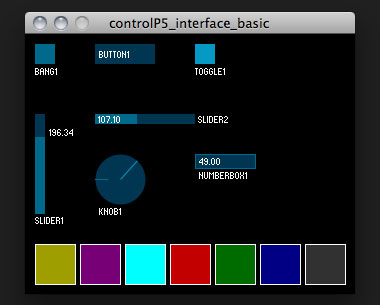
\includegraphics[width=8cm]{gambar/controlp5.jpg}
	\caption{Grafik Pengujian Koordinat X}
	\label{pic.koordinatx}
\end{figure}

Dari hasil pengujian yang ditampilkan pada Tabel \ref{tbl.koordinatx} dan juga Gambar \ref{pic.koordinatx} terlihat bahwa posisi \textit{end-effector} yang dihasilkan pada robot SCARA dibandingkan dengan data sesuai perhitungan kinematika memiliki sedikit perbedaan pada beberapa data. Perbedaan data ini dapat ditolerasi karena dengan \textit{sampling} koordinat $x$ yang diuji hanya kurang dari lima persen nilai data yang berbeda. Pada hasil yang ditunjukkan diketahui bahwa posisi \textit{end-effector} memiliki batas minimum dan juga maksimum. Batas minimum posisi \textit{end-effector} pada sumbu $x$ yaitu ? cm dari titik pusat dan batas maksimum posisi \textit{end-effector} pada posisi sumbu $x$ adalah ? cm yang merupakan panjang dari lengan \textit{shoulder} dan juga lengan \textit{elbow}. 

\subsubsection{Pengujian Koordinat Y}
Pengujian koordinat $y$ dilakukan untuk mengetahui batas minimal dan batas maksimal \textit{end-effector} dari \textit{arm manipulator} robot SCARA relatif terhadap sumbu $y$. Pengujian koordinat $y$ dilakukan dengan cara mengujicobakan setiap titik dari ? cm sampai dengan total panjang \textit{shoulder} dan \textit{elbow} yaitu ? cm menggunakan perhitungan kinematika balik. Perhitungan posisi $y$ diujicobakan menggunakan program Processing IDE, sementara untuk pengukuran posisi diukur secara faktual dari posisi \textit{end-effector} dengan membuat sebuah diagram kartesius. Tabel \ref{tbl.koordinaty} menunjukkan pengujian koordinat $y$ dan Gambar \ref{pic.koordinaty} menunjukkan grafik dari \textit{sampling} koordinat $y$.
 \begin{table}[H]
 	\centering
 	\caption{Hasil Pengujian Koordinat Y}
 	\label{tbl.koordinaty}
 	\begin{tabular}{|c|l|}
 		\hline
 		\rowcolor[HTML]{9B9B9B} 
 		
 		No & \multicolumn{1}{c|}{\cellcolor[HTML]{9B9B9B}Keterangan} \\ \hline
 		1  & Robot Lengan SCARA                                      \\ \hline
 		2  & Box Panel                                               \\ \hline
 		3  & Arduino Mega 2560                                       \\ \hline
 		4  & Personal Computer                                       \\ \hline
 		5  & GUI Processing IDE                                      \\ \hline
 		6  & Workspace Robot SCARA                                   \\ \hline
 		7  & Kompresor                                               \\ \hline
 		8  & Objek                                                   \\ \hline
 	\end{tabular}
 	
 \end{table} 
 \begin{figure}[H]
 	\centering
 	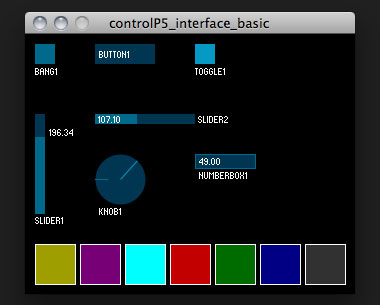
\includegraphics[width=8cm]{gambar/controlp5.jpg}
 	\caption{Grafik Pengujian Koordinat Y}
 	\label{pic.koordinaty}
 \end{figure}


Dari hasil pengujian yang ditampilkan pada Tabel \ref{tbl.koordinaty} dan juga Gambar \ref{pic.koordinaty} terlihat bahwa posisi \textit{end-effector} yang dihasilkan pada robot SCARA dibandingkan dengan data sesuai perhitungan kinematika memiliki sedikit perbedaan pada beberapa data. Perbedaan data ini dapat ditolerasi karena dengan \textit{sampling} koordinat $y$ yang diuji hanya kurang dari lima persen nilai data yang berbeda. Pada hasil yang ditunjukkan diketahui bahwa posisi \textit{end-effector} memiliki batas minimum dan juga maksimum. Batas minimum posisi \textit{end-effector} pada sumbu $x$ yaitu ? cm dari titik pusat dan batas maksimum posisi \textit{end-effector} pada posisi sumbu $y$ adalah ? cm yang merupakan panjang dari lengan \textit{shoulder} dan juga lengan \textit{elbow}. 

\subsubsection{Pengujian \textit{Joint Shoulder}}
Pengujian \textit{joint shoulder} dilakukan dengan membandingkan nilai sudut yang dihasilkan oleh perhitungan kinematika yang ada pada program Processing IDE dengan sudut yang dihasilkan dalam aktual robot SCARA. Pengujian dilakukan dengan cara memberikan sebuah posisi koordinat $x$ dan $y$ dengan nilai yang bervariasi. Nilai tersebut dimasukkan ke dalam sebuah perhitungan kinematika balik yang ada pada program Processing IDE sesuai dengan persamaan pada bab sebelumnya. Hasil yang dihasilkan oleh perhitungan merupakan nilai sudut dari \textit{joint shoulder} dan juga \textit{elbow}. Perhitungan aktual dilakukan dengan cara mengukur sudut pada setiap \textit{joint} menggunakan bantuan busur atau \textit{software} sensor kemiringan yang di-\textit{install} pada smartphone. Tabel \ref{tbl.jointshoudler} merupakan hasil pengujian dari \textit{joint shoulder} berdasarkan \textit{sampling} posisi yang diambil. Gambar \ref{pic.jointshoulder} merupakan grafik hubungan dari sudut aktual dan sudut berdasarkan perhitungan kinematika. 

\begin{table}[H]
	\centering
	\caption{Hasil Pengujian \textit{Joint Shoulder}}
	\label{tbl.jointshoulder}
	\begin{tabular}{|c|l|}
		\hline
		\rowcolor[HTML]{9B9B9B} 
		
		No & \multicolumn{1}{c|}{\cellcolor[HTML]{9B9B9B}Keterangan} \\ \hline
		1  & Robot Lengan SCARA                                      \\ \hline
		2  & Box Panel                                               \\ \hline
		3  & Arduino Mega 2560                                       \\ \hline
		4  & Personal Computer                                       \\ \hline
		5  & GUI Processing IDE                                      \\ \hline
		6  & Workspace Robot SCARA                                   \\ \hline
		7  & Kompresor                                               \\ \hline
		8  & Objek                                                   \\ \hline
	\end{tabular}
	
\end{table} 
\begin{figure}[H]
	\centering
	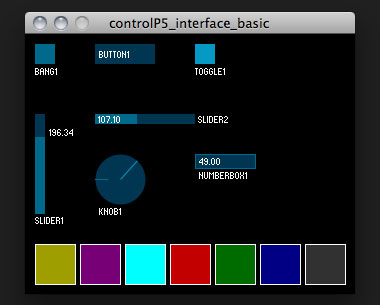
\includegraphics[width=8cm]{gambar/controlp5.jpg}
	\caption{Grafik Pengujian \textit{Joint Shoulder}}
	\label{pic.jointshoulder}
\end{figure}

Pada hasil yang ditunjukkan oleh Tabel \ref{tbl.jointshoulder} dan Gambar \ref{pic.jointshoulder} terlihat bahwa secara keseleuruhan nilai sudut yang dihasilkan oleh aktual pada robot SCARA dibandingkan dengan perhitungan kinematika oleh Processing IDE tidak begitu terdapat perbedaan. Terlihat bahwa nilai error
 memiliki nilai minimum .... persen dan nilai maksimum ... persen. Persentase error didapat dari data yang tidak sesuai dibagi oleh keleluruhan data yang diuji coba. Dapat dikatakan bahwa pengujian sudut \textit{joint shoulder} cukup baik.
 
 \subsubsection{Pengujian \textit{Joint Elbow}}
 Pengujian \textit{joint elbow} dilakukan dengan membandingkan nilai sudut yang dihasilkan oleh perhitungan kinematika yang ada pada program Processing IDE dengan sudut yang dihasilkan dalam aktual robot SCARA. Pengujian dilakukan dengan cara memberikan sebuah posisi koordinat $x$ dan $y$ dengan nilai yang bervariasi. Nilai tersebut dimasukkan ke dalam sebuah perhitungan kinematika balik yang ada pada program Processing IDE. Hasil yang dihasilkan oleh perhitungan merupakan nilai sudut dari \textit{joint shoulder} dan juga \textit{elbow}. Perhitungan aktual dilakukan dengan cara mengukur sudut pada setiap \textit{joint} menggunakan bantuan busur atau \textit{software} sensor kemiringan yang di-\textit{install} pada smartphone. Tabel \ref{tbl.jointelbow} merupakan hasil pengujian dari \textit{joint elbow} berdasarkan \textit{sampling} posisi yang diambil. Gambar \ref{pic.jointelbow} merupakan grafik hubungan dari sudut aktual dan sudut berdasarkan perhitungan kinematika. 
 
 \begin{table}[H]
 	\centering
 	\caption{Hasil Pengujian \textit{Joint Elbow}}
 	\label{tbl.jointelbow}
 	\begin{tabular}{|c|l|}
 		\hline
 		\rowcolor[HTML]{9B9B9B} 
 		
 		No & \multicolumn{1}{c|}{\cellcolor[HTML]{9B9B9B}Keterangan} \\ \hline
 		1  & Robot Lengan SCARA                                      \\ \hline
 		2  & Box Panel                                               \\ \hline
 		3  & Arduino Mega 2560                                       \\ \hline
 		4  & Personal Computer                                       \\ \hline
 		5  & GUI Processing IDE                                      \\ \hline
 		6  & Workspace Robot SCARA                                   \\ \hline
 		7  & Kompresor                                               \\ \hline
 		8  & Objek                                                   \\ \hline
 	\end{tabular}
 	
 \end{table} 
 \begin{figure}[H]
 	\centering
 	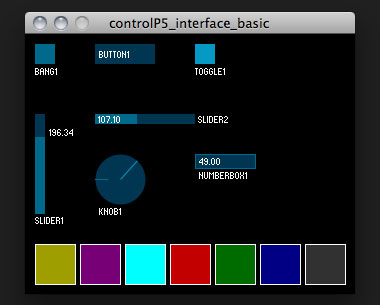
\includegraphics[width=8cm]{gambar/controlp5.jpg}
 	\caption{Grafik Pengujian \textit{Joint Elbow}}
 	\label{pic.jointelbow}
 \end{figure}
 
 Pada hasil yang ditunjukkan oleh Tabel \ref{tbl.jointelbow} dan Gambar \ref{pic.jointelbow} terlihat bahwa secara keseleuruhan nilai sudut yang dihasilkan oleh aktual pada robot SCARA dibandingkan dengan perhitungan kinematika oleh Processing IDE tidak begitu terdapat perbedaan. Terlihat bahwa nilai error
 memiliki nilai minimum .... persen dan nilai maksimum ... persen. Persentase error didapat dari data yang tidak sesuai dibagi oleh keleluruhan data yang diuji coba. Nilai tersebut dapat ditoleransi dan pengujian sudut \textit{joint elbow} dapat dikatakan baik.
 \subsection{Pengujian GUI}
 Pengujian GUI dilakukan untuk membandingkan posisi dari aktual robot SCARA dengan posisi yang ada pada Processing IDE. Pengujian dilakukan dengan memberikan \textit{sampling} posisi yang kemudian dilihat posisi dari robot secara aktual maupun Processing IDE. Gambar \ref{pic.pengujiangui1}, Gambar \ref{pic.pengujiangui2}, dan Gambar \ref{pic.pengujiangui3} merupakan hasil \textit{sampling} perbandingan posisi dari robot SCARA secara aktual dan secara animasi.
  \begin{figure}[H]
 	\centering
 	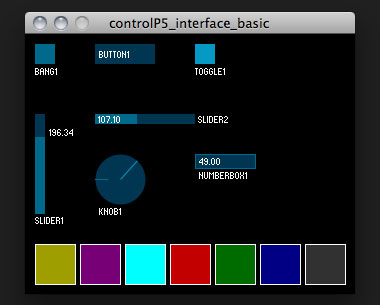
\includegraphics[width=8cm]{gambar/controlp5.jpg}
 	\caption{Perbandingan Gambaran Robot SCARA}
 	\label{pic.pengujiangui1}
 \end{figure}
\begin{figure}[H]
	\centering
	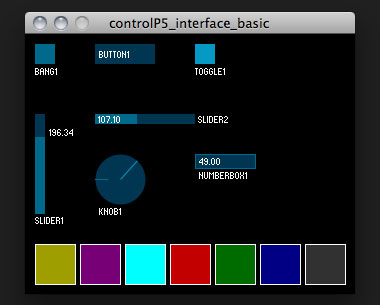
\includegraphics[width=8cm]{gambar/controlp5.jpg}
	\caption{Perbandingan Gambaran Robot SCARA}
	\label{pic.pengujiangui2}
\end{figure}
\begin{figure}[H]
	\centering
	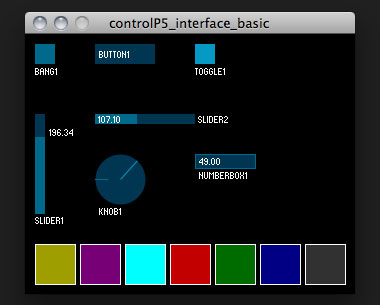
\includegraphics[width=8cm]{gambar/controlp5.jpg}
	\caption{Perbandingan Gambaran Robot SCARA}
	\label{pic.pengujiangui3}
\end{figure}
Dari hasil yang ditunjukkan oleh Gambar \ref{pic.pengujiangui1}, Gambar \ref{pic.pengujiangui2}, dan Gambar \ref{pic.pengujiangui3} terlihat bahwa perbedaan posisi dari robot SCARA aktual dan pada Processing IDE hanya beberapa dan dapat ditoleransi, Terlihat bahwa posisi koordinat\textit{ end-effector }yang ditunjukkan oleh robot SCARA aktual dan robot SCARA processing IDE terlihat beberapa perbedaan yang masih dapat ditoleransi. Sudut dari \textit{shoulder} dan \textit{elbow} yang masing-masing ditunjukkan terlihat sama. Dengan begitu, pengujian GUI dapat dikatakan baik.

\section{Pengujian Keseluruhan}
Setelah semua komponen sistem yang diuji dapat bekerja dengan baik, pengujian selanjutnya adalah pengujian sistem secara keseluruhan dengan beberapa parameter uji yang diberikan. Parameter uji tersebut diantaranya adalah pengujian akurasi robot lengan, dan simulasi robot lengan. 

\subsection{Pengujian Akurasi Robot Lengan}
Pada pengujian akurasi robot lengan dilakukan pengujian dengan memberikan posisi koordinat $x$ dan $y$ dan melihat kembali posisi $x$ dan $y$ secara aktual, melihat besar sudut pada masing-masing joint dengan perbandingan perhitungan kinematika. Pengujian akurasi robot lengan ini akan menghasilkan sebuah hasil secara luas dan dapat ditarik untuk sebuah kesimpulan yang menentukan robot SCARA dapat bekerja baik atau buruk secara keseluruhan. Tabel \ref{tbl.akurasikeseluruhan} merupakan hasil dari pengujian akurasi robot lengan secara keseluruhan. Gambar \ref{pic.akurasikeseluruhan} merupakan grafik dari hasil pengujian akurasi robot lengan secara keseluruhan.

\begin{table}[H]
	\centering
	\caption{Hasil Pengujian Akurasi Robot Secara Keseluruhan}
	\label{tbl.akurasikeseluruhan}
	\begin{tabular}{|c|l|}
		\hline
		\rowcolor[HTML]{9B9B9B} 
		
		No & \multicolumn{1}{c|}{\cellcolor[HTML]{9B9B9B}Keterangan} \\ \hline
		1  & Robot Lengan SCARA                                      \\ \hline
		2  & Box Panel                                               \\ \hline
		3  & Arduino Mega 2560                                       \\ \hline
		4  & Personal Computer                                       \\ \hline
		5  & GUI Processing IDE                                      \\ \hline
		6  & Workspace Robot SCARA                                   \\ \hline
		7  & Kompresor                                               \\ \hline
		8  & Objek                                                   \\ \hline
	\end{tabular}
	
\end{table} 
\begin{figure}[H]
	\centering
	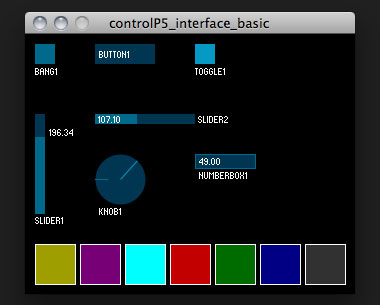
\includegraphics[width=8cm]{gambar/controlp5.jpg}
	\caption{Grafik Pengujian Akurasi Robot Secara Keseluruhan}
	\label{pic.akurasikeseluruhan}
\end{figure}

Pada hasil pengujian yang ditunjukkan pada Tabel \ref{tbl.akurasikeseluruhan} dan Gambar \ref{pic.akurasikeseluruhan} terlihat bahwa pengujian mendapat beberapa data yang beragam. Terlihat bahwa nilai kesalahan paling banyak terdapat pada bagian posisi koordinat $x$ dan $y$ dan kesalahan paling sedikit pada bagian sudut \textit{shoulder}. Sedangkan untuk sistem keseluruhan kesalahan total pada akurasi robot memiliki nilai ... persen. Nilai sebesar ini merupakan nilai yang cukup baik bagi sebuah sistem. Dengan nilai tersebut maka sistem kinematika robot SCARA ini dapat dikatakan baik. 
\subsection{Pengujian Simulasi Robot Lengan}
Pada pengujian ini, dilakukan serangkaian simulasi robot lengan untuk melakukan pergerakan sesuai dengan data yang diberikan melalui GUI yang telah dibuat. Simulasi ini menggunakan semua komponen yang ada di dalam perancangan, diantaranya robot SCARA, \textit{workspace}, catu daya, komputer personal, GUI Processing IDE, dan objek.

Pertama, robot SCARA berada posisi normal yang berarti pada posisi lurus searah dengan sumbu $y$. Robot SCARA akan mulai bergerak pada saat nilai data pada Processing IDE telah didapatkan dan kemudian dikirimkan ke Arduino Mega 2560. Proses pemilihan data pada Processing IDE dilalui pada sebuah GUI yang telah dibuat sesuai dengan fungsi dari robot SCARA. Pada GUI terdapat beberapa pilihan dalam memberikan sebuah nilai masukan. 

Kedua, robot SCARA akan mulai bergerak menuju posisi seperti data yang dimasukkan dan kemudian berhenti pada posisi tersebut dan mengambil objek yang dibawa oleh \textit{end-effector} pada posisi akhir.  Pergerakan \textit{end-effector} ditenagai oleh tekanan udara pada sebuah kompresor yang dikontrol oleh\textit{ valve pneumatic} yang diotaki oleh TIP31. Posisi akhir merupakan posisi dimana semua objek dikumpulkan. Setelah melakukan satu pekerjaan tersebut, robot SCARA kembali pada posisi normal dan menunggu data yang diberikan kembali oleh Processing IDE.  Gambar \ref{pic.simulasiakhir} merupakan simulasi robot lengan SCARA menggunakan masukan pada GUI yang telah dibuat.
 \begin{figure}[H]
 	\centering
 	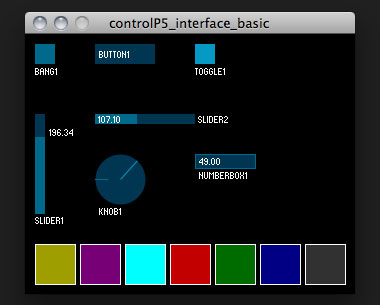
\includegraphics[width=8cm]{gambar/controlp5.jpg}
 	\caption{Simulasi Robot Lengan Menggunakan GUI }
 	\label{pic.simulasiakhir}
 \end{figure}




